% --------------------------------------------------------------------------- %
%                       _           _
%   ___ ___  _ __   ___| |_   _  __| | ___
%  / __/ _ \| '_ \ / __| | | | |/ _` |/ _ \
% | (_| (_) | | | | (__| | |_| | (_| |  __/
%  \___\___/|_| |_|\___|_|\__,_|\__,_|\___|
% --------------------------------------------------------------------------- %
\chapter{Conclusion}{Embracing AR within Computational Art and Music}
\label{sec: conclusion}
%\markboth{}{Conclusion}
\epigraph{\textit{`The image with which the artist works to realise his or her idea is no longer a phantom, it can be touched, navigated and negotiated with.'}}{\citep[p.5]{ryan1991}}

% \begin{figure}
%     \centering
%     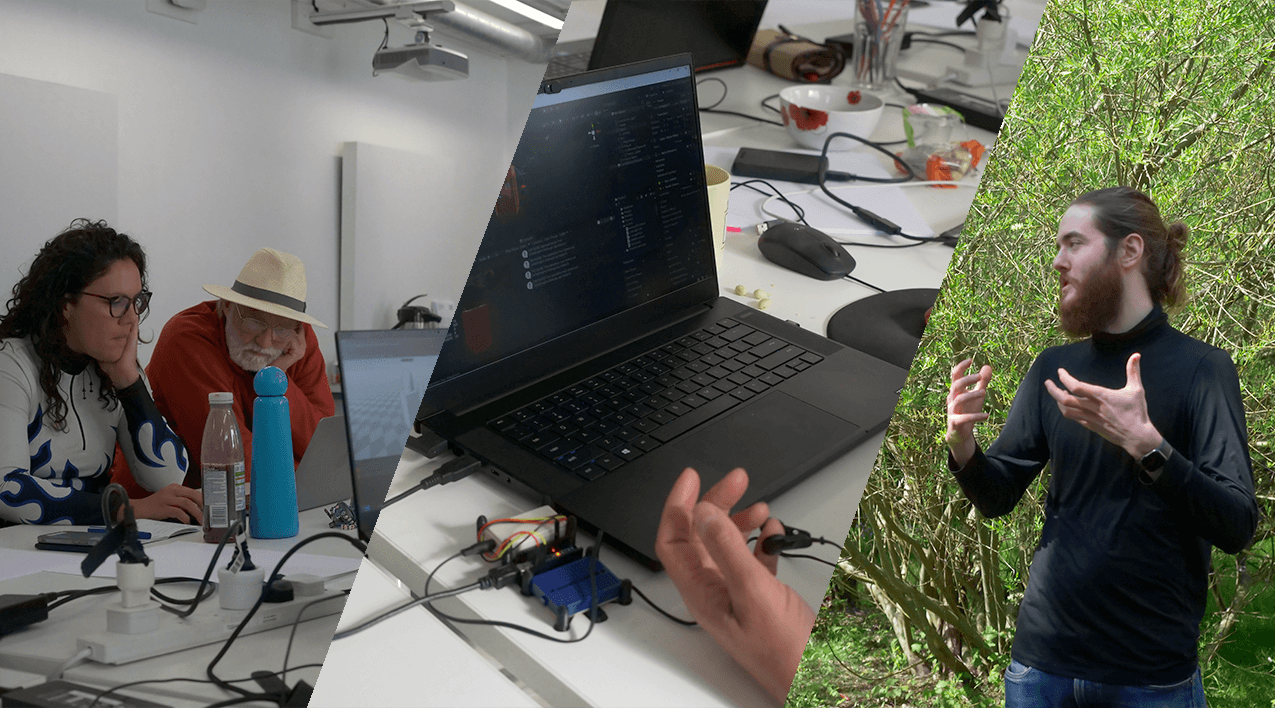
\includegraphics[width=1\linewidth]{0x-x/chapter-fig.png}
%     \captionsetup{labelformat=empty}
%     \caption[\autoref{sec: x}: x, (from \citeauthor{x}, \citeyear{x})]{}
% \end{figure}

\clearpage
% --------------------------------------------------------------------------- %

\section{Summary}\label{sec: conclusion-summary}
There is no doubt, that AR is one of the most exciting forms of technology on our horizon as artists and musicians. In this thesis, I hope I have portrayed this, with sufficient rationale, and explanation. However, there do exist significant problems; its origin in the U.S. military-industrial complex, as a tool for enabling neo-colonialism and the streamlining of workforces by increasing efficiency. Moreover, the threat of mega-corporations on our digital freedom, safety, and rights to privacy is beginning to surface in discussions regarding `the Metaverse' - the supposed site of XR development. In stark contrast, federated and open communities like those that ActivityPub and Matrix provide, enable new and exciting ways to shift away from these platforms and the algorithmic harm they inflict. As such, open-source tools have provided much of the ability to carry out this research, and I would again like to thank those in the community that have helped: namely those involved in the Project North Star, LibPdIntegration teams.

The present thesis has presented three practical contributions to embodied musical knowledge and understanding in the form of \textit{\hyperref[sec: area]{area\textasciitilde{}}}, \textit{\hyperref[sec: polaris]{polaris\textasciitilde{}}}, and \textit{\hyperref[sec: polygons]{polygons\textasciitilde{}}}. In addition it has provided a set of three theoretical propositions, termed: augmented \hyperref[sec: discussion-medium-material]{materiality}, \hyperref[sec: discussion-medium-embodiment]{embodiment}, and \hyperref[sec: discussion-medium-space]{space} From this, design patterns for those in the field interested in reproducing or developing similar works, namely: \textit{\nameref{sec: discussion-patterns-experience}}, \textit{\nameref{sec: discussion-patterns-instrument}}, and \textit{\nameref{sec: discussion-patterns-environment}}, have been developed and shared. 

\section{Future Work}\label{sec: conclusion-futurework}
It is my hope to carry on developing expressive tools for musical creativity long into the future, and these will be located on \href{https://sambilbow.com}{on my website}. In \textit{\nameref{sec: polygons}}, I remarked on the work that was outstanding in developing a sound ARt performance practice. It is my hope in the near future, to develop a set of tools for artists and musicians interested in collective forms of AR headset expression, with a project entitled CoMuSe: Collective Musical Sensehacking. This will explore `multiplayer' or ensemble sound ARt performances.
